% Options for packages loaded elsewhere
\PassOptionsToPackage{unicode}{hyperref}
\PassOptionsToPackage{hyphens}{url}
\PassOptionsToPackage{dvipsnames,svgnames,x11names}{xcolor}
%
\documentclass[
  letterpaper,
  DIV=11,
  numbers=noendperiod]{scrartcl}

\usepackage{amsmath,amssymb}
\usepackage{iftex}
\ifPDFTeX
  \usepackage[T1]{fontenc}
  \usepackage[utf8]{inputenc}
  \usepackage{textcomp} % provide euro and other symbols
\else % if luatex or xetex
  \usepackage{unicode-math}
  \defaultfontfeatures{Scale=MatchLowercase}
  \defaultfontfeatures[\rmfamily]{Ligatures=TeX,Scale=1}
\fi
\usepackage{lmodern}
\ifPDFTeX\else  
    % xetex/luatex font selection
\fi
% Use upquote if available, for straight quotes in verbatim environments
\IfFileExists{upquote.sty}{\usepackage{upquote}}{}
\IfFileExists{microtype.sty}{% use microtype if available
  \usepackage[]{microtype}
  \UseMicrotypeSet[protrusion]{basicmath} % disable protrusion for tt fonts
}{}
\makeatletter
\@ifundefined{KOMAClassName}{% if non-KOMA class
  \IfFileExists{parskip.sty}{%
    \usepackage{parskip}
  }{% else
    \setlength{\parindent}{0pt}
    \setlength{\parskip}{6pt plus 2pt minus 1pt}}
}{% if KOMA class
  \KOMAoptions{parskip=half}}
\makeatother
\usepackage{xcolor}
\setlength{\emergencystretch}{3em} % prevent overfull lines
\setcounter{secnumdepth}{-\maxdimen} % remove section numbering
% Make \paragraph and \subparagraph free-standing
\ifx\paragraph\undefined\else
  \let\oldparagraph\paragraph
  \renewcommand{\paragraph}[1]{\oldparagraph{#1}\mbox{}}
\fi
\ifx\subparagraph\undefined\else
  \let\oldsubparagraph\subparagraph
  \renewcommand{\subparagraph}[1]{\oldsubparagraph{#1}\mbox{}}
\fi

\usepackage{color}
\usepackage{fancyvrb}
\newcommand{\VerbBar}{|}
\newcommand{\VERB}{\Verb[commandchars=\\\{\}]}
\DefineVerbatimEnvironment{Highlighting}{Verbatim}{commandchars=\\\{\}}
% Add ',fontsize=\small' for more characters per line
\usepackage{framed}
\definecolor{shadecolor}{RGB}{241,243,245}
\newenvironment{Shaded}{\begin{snugshade}}{\end{snugshade}}
\newcommand{\AlertTok}[1]{\textcolor[rgb]{0.68,0.00,0.00}{#1}}
\newcommand{\AnnotationTok}[1]{\textcolor[rgb]{0.37,0.37,0.37}{#1}}
\newcommand{\AttributeTok}[1]{\textcolor[rgb]{0.40,0.45,0.13}{#1}}
\newcommand{\BaseNTok}[1]{\textcolor[rgb]{0.68,0.00,0.00}{#1}}
\newcommand{\BuiltInTok}[1]{\textcolor[rgb]{0.00,0.23,0.31}{#1}}
\newcommand{\CharTok}[1]{\textcolor[rgb]{0.13,0.47,0.30}{#1}}
\newcommand{\CommentTok}[1]{\textcolor[rgb]{0.37,0.37,0.37}{#1}}
\newcommand{\CommentVarTok}[1]{\textcolor[rgb]{0.37,0.37,0.37}{\textit{#1}}}
\newcommand{\ConstantTok}[1]{\textcolor[rgb]{0.56,0.35,0.01}{#1}}
\newcommand{\ControlFlowTok}[1]{\textcolor[rgb]{0.00,0.23,0.31}{#1}}
\newcommand{\DataTypeTok}[1]{\textcolor[rgb]{0.68,0.00,0.00}{#1}}
\newcommand{\DecValTok}[1]{\textcolor[rgb]{0.68,0.00,0.00}{#1}}
\newcommand{\DocumentationTok}[1]{\textcolor[rgb]{0.37,0.37,0.37}{\textit{#1}}}
\newcommand{\ErrorTok}[1]{\textcolor[rgb]{0.68,0.00,0.00}{#1}}
\newcommand{\ExtensionTok}[1]{\textcolor[rgb]{0.00,0.23,0.31}{#1}}
\newcommand{\FloatTok}[1]{\textcolor[rgb]{0.68,0.00,0.00}{#1}}
\newcommand{\FunctionTok}[1]{\textcolor[rgb]{0.28,0.35,0.67}{#1}}
\newcommand{\ImportTok}[1]{\textcolor[rgb]{0.00,0.46,0.62}{#1}}
\newcommand{\InformationTok}[1]{\textcolor[rgb]{0.37,0.37,0.37}{#1}}
\newcommand{\KeywordTok}[1]{\textcolor[rgb]{0.00,0.23,0.31}{#1}}
\newcommand{\NormalTok}[1]{\textcolor[rgb]{0.00,0.23,0.31}{#1}}
\newcommand{\OperatorTok}[1]{\textcolor[rgb]{0.37,0.37,0.37}{#1}}
\newcommand{\OtherTok}[1]{\textcolor[rgb]{0.00,0.23,0.31}{#1}}
\newcommand{\PreprocessorTok}[1]{\textcolor[rgb]{0.68,0.00,0.00}{#1}}
\newcommand{\RegionMarkerTok}[1]{\textcolor[rgb]{0.00,0.23,0.31}{#1}}
\newcommand{\SpecialCharTok}[1]{\textcolor[rgb]{0.37,0.37,0.37}{#1}}
\newcommand{\SpecialStringTok}[1]{\textcolor[rgb]{0.13,0.47,0.30}{#1}}
\newcommand{\StringTok}[1]{\textcolor[rgb]{0.13,0.47,0.30}{#1}}
\newcommand{\VariableTok}[1]{\textcolor[rgb]{0.07,0.07,0.07}{#1}}
\newcommand{\VerbatimStringTok}[1]{\textcolor[rgb]{0.13,0.47,0.30}{#1}}
\newcommand{\WarningTok}[1]{\textcolor[rgb]{0.37,0.37,0.37}{\textit{#1}}}

\providecommand{\tightlist}{%
  \setlength{\itemsep}{0pt}\setlength{\parskip}{0pt}}\usepackage{longtable,booktabs,array}
\usepackage{calc} % for calculating minipage widths
% Correct order of tables after \paragraph or \subparagraph
\usepackage{etoolbox}
\makeatletter
\patchcmd\longtable{\par}{\if@noskipsec\mbox{}\fi\par}{}{}
\makeatother
% Allow footnotes in longtable head/foot
\IfFileExists{footnotehyper.sty}{\usepackage{footnotehyper}}{\usepackage{footnote}}
\makesavenoteenv{longtable}
\usepackage{graphicx}
\makeatletter
\def\maxwidth{\ifdim\Gin@nat@width>\linewidth\linewidth\else\Gin@nat@width\fi}
\def\maxheight{\ifdim\Gin@nat@height>\textheight\textheight\else\Gin@nat@height\fi}
\makeatother
% Scale images if necessary, so that they will not overflow the page
% margins by default, and it is still possible to overwrite the defaults
% using explicit options in \includegraphics[width, height, ...]{}
\setkeys{Gin}{width=\maxwidth,height=\maxheight,keepaspectratio}
% Set default figure placement to htbp
\makeatletter
\def\fps@figure{htbp}
\makeatother

\usepackage{booktabs}
\usepackage{longtable}
\usepackage{array}
\usepackage{multirow}
\usepackage{wrapfig}
\usepackage{float}
\usepackage{colortbl}
\usepackage{pdflscape}
\usepackage{tabu}
\usepackage{threeparttable}
\usepackage{threeparttablex}
\usepackage[normalem]{ulem}
\usepackage{makecell}
\usepackage{xcolor}
\KOMAoption{captions}{tableheading}
\makeatletter
\@ifpackageloaded{caption}{}{\usepackage{caption}}
\AtBeginDocument{%
\ifdefined\contentsname
  \renewcommand*\contentsname{Table of contents}
\else
  \newcommand\contentsname{Table of contents}
\fi
\ifdefined\listfigurename
  \renewcommand*\listfigurename{List of Figures}
\else
  \newcommand\listfigurename{List of Figures}
\fi
\ifdefined\listtablename
  \renewcommand*\listtablename{List of Tables}
\else
  \newcommand\listtablename{List of Tables}
\fi
\ifdefined\figurename
  \renewcommand*\figurename{Figure}
\else
  \newcommand\figurename{Figure}
\fi
\ifdefined\tablename
  \renewcommand*\tablename{Table}
\else
  \newcommand\tablename{Table}
\fi
}
\@ifpackageloaded{float}{}{\usepackage{float}}
\floatstyle{ruled}
\@ifundefined{c@chapter}{\newfloat{codelisting}{h}{lop}}{\newfloat{codelisting}{h}{lop}[chapter]}
\floatname{codelisting}{Listing}
\newcommand*\listoflistings{\listof{codelisting}{List of Listings}}
\makeatother
\makeatletter
\makeatother
\makeatletter
\@ifpackageloaded{caption}{}{\usepackage{caption}}
\@ifpackageloaded{subcaption}{}{\usepackage{subcaption}}
\makeatother
\ifLuaTeX
  \usepackage{selnolig}  % disable illegal ligatures
\fi
\usepackage{bookmark}

\IfFileExists{xurl.sty}{\usepackage{xurl}}{} % add URL line breaks if available
\urlstyle{same} % disable monospaced font for URLs
\hypersetup{
  pdftitle={Lab 4: Data Transformations},
  pdfauthor={Darwhin Gomez},
  colorlinks=true,
  linkcolor={blue},
  filecolor={Maroon},
  citecolor={Blue},
  urlcolor={Blue},
  pdfcreator={LaTeX via pandoc}}

\title{Lab 4: Data Transformations}
\author{Darwhin Gomez}
\date{}

\begin{document}
\maketitle

\subsection{Overview: Large Technology
Stocks}\label{overview-large-technology-stocks}

For this assignment we practice data transformation using a dataset of
the daily prices and daily trading volumes of a group of large
technology stocks that trade on US stock exchanges.
\href{https://github.com/georgehagstrom/DATA607/tree/main/website/assignments/labs/labData/stocks.csv}{Click
here to download stocks.csv}, which contains data going back to 2000.
The dataset contains several variables, including:

\begin{itemize}
\tightlist
\item
  \texttt{symbol}: which is the ticker symbol for the stock
\item
  \texttt{date}: which is the trading date
\item
  \texttt{open}, \texttt{high}, \texttt{low}, and \texttt{close}, which
  are the price at the start of trading, the high price during the day,
  the low price during the day, and the stock price at the close of
  trading (unit is USD)
\item
  \texttt{adjusted}: which is the stock price at close adjusted for the
  financial effects of special events (such as dividends). Unit is USD
\item
  \texttt{volume}: which is the number of shares which traded during a
  given trading day.
\end{itemize}

\begin{Shaded}
\begin{Highlighting}[]
\FunctionTok{library}\NormalTok{(tidyverse)}
\FunctionTok{library}\NormalTok{(TTR)}
\FunctionTok{library}\NormalTok{(kableExtra)}

\NormalTok{stocks }\OtherTok{=} \FunctionTok{read\_csv}\NormalTok{(}\StringTok{"stocks.csv"}\NormalTok{)}

\NormalTok{stocks }\SpecialCharTok{|\textgreater{}} \FunctionTok{head}\NormalTok{(}\DecValTok{10}\NormalTok{) }\SpecialCharTok{|\textgreater{}} \FunctionTok{kable}\NormalTok{()}
\end{Highlighting}
\end{Shaded}

\begin{longtable}[]{@{}
  >{\raggedright\arraybackslash}p{(\columnwidth - 14\tabcolsep) * \real{0.0933}}
  >{\raggedright\arraybackslash}p{(\columnwidth - 14\tabcolsep) * \real{0.1467}}
  >{\raggedleft\arraybackslash}p{(\columnwidth - 14\tabcolsep) * \real{0.1200}}
  >{\raggedleft\arraybackslash}p{(\columnwidth - 14\tabcolsep) * \real{0.1200}}
  >{\raggedleft\arraybackslash}p{(\columnwidth - 14\tabcolsep) * \real{0.1200}}
  >{\raggedleft\arraybackslash}p{(\columnwidth - 14\tabcolsep) * \real{0.1200}}
  >{\raggedleft\arraybackslash}p{(\columnwidth - 14\tabcolsep) * \real{0.1467}}
  >{\raggedleft\arraybackslash}p{(\columnwidth - 14\tabcolsep) * \real{0.1333}}@{}}
\toprule\noalign{}
\begin{minipage}[b]{\linewidth}\raggedright
symbol
\end{minipage} & \begin{minipage}[b]{\linewidth}\raggedright
date
\end{minipage} & \begin{minipage}[b]{\linewidth}\raggedleft
open
\end{minipage} & \begin{minipage}[b]{\linewidth}\raggedleft
high
\end{minipage} & \begin{minipage}[b]{\linewidth}\raggedleft
low
\end{minipage} & \begin{minipage}[b]{\linewidth}\raggedleft
close
\end{minipage} & \begin{minipage}[b]{\linewidth}\raggedleft
volume
\end{minipage} & \begin{minipage}[b]{\linewidth}\raggedleft
adjusted
\end{minipage} \\
\midrule\noalign{}
\endhead
\bottomrule\noalign{}
\endlastfoot
AAPL & 2000-01-03 & 0.936384 & 1.004464 & 0.907924 & 0.999442 &
535796800 & 0.8440041 \\
AAPL & 2000-01-04 & 0.966518 & 0.987723 & 0.903460 & 0.915179 &
512377600 & 0.7728457 \\
AAPL & 2000-01-05 & 0.926339 & 0.987165 & 0.919643 & 0.928571 &
778321600 & 0.7841553 \\
AAPL & 2000-01-06 & 0.947545 & 0.955357 & 0.848214 & 0.848214 &
767972800 & 0.7162958 \\
AAPL & 2000-01-07 & 0.861607 & 0.901786 & 0.852679 & 0.888393 &
460734400 & 0.7502258 \\
AAPL & 2000-01-10 & 0.910714 & 0.912946 & 0.845982 & 0.872768 &
505064000 & 0.7370310 \\
AAPL & 2000-01-11 & 0.856585 & 0.887277 & 0.808036 & 0.828125 &
441548800 & 0.6993311 \\
AAPL & 2000-01-12 & 0.848214 & 0.852679 & 0.772321 & 0.778460 &
976068800 & 0.6573902 \\
AAPL & 2000-01-13 & 0.843610 & 0.881696 & 0.825893 & 0.863839 &
1032684800 & 0.7294905 \\
AAPL & 2000-01-14 & 0.892857 & 0.912946 & 0.887277 & 0.896763 &
390376000 & 0.7572942 \\
\end{longtable}

All of the the stock prices and the trading volume have been adjusted
for stock splits, so that the data provide a continuous record of how
prices and trading volume changed.

There are several important functions and packages that you will need to
use to complete this exercise.

\begin{itemize}
\tightlist
\item
  We will make a lot of use of window functions in \texttt{dplyr}, which
  are very helpful for making transformations (including \texttt{lead},
  \texttt{lag}, \texttt{percent\_rank}). The
  \href{https://dplyr.tidyverse.org/articles/window-functions.html}{\texttt{dplyr}
  vignettes and articles are incredibly useful for learning about all
  the different functions available}
\item
  We will use the \texttt{TTR} package (which is part of the
  \texttt{tidyquant} family of packages,
  \href{https://cran.r-project.org/web/packages/tidyquant/vignettes/TQ02-quant-integrations-in-tidyquant.html}{see
  here}). The main function we will use is called \texttt{runMean}. An
  alternative package that is also very nice but not part of the
  \texttt{tidyverse} is
  \href{https://CRAN.R-project.org/package=RcppRoll}{\texttt{RcppRoll}}
\item
  If you aren't very comfortable with logarithms, you should read more
  about them. They are one of the most important mathematical functions
  for data science. We aren't using their mathematical properties much
  this week but they will be important throughout your data science
  journey.
  \href{https://www.khanacademy.org/math/algebra2/x2ec2f6f830c9fb89:logs/x2ec2f6f830c9fb89:log-intro/v/logarithms}{Khan
  Academy has a decent video}, and
  \href{https://www.nature.com/articles/news.2008.866}{this article in
  the journal nature} has some more context.
\item
  We will calculate some correlation coefficients, using the
  \texttt{cor} function from base R (\texttt{?cor} to see how it is
  used). There is also a \texttt{tidyverse} package called
  \texttt{corrr} that is useful for calculating correlations on data
  frames, but we won't use it for this lab.
\item
  The motivation for today's assignment came from some news articles a
  few years ago about how big tech stocks collectively had a miniature
  meltdown after powering the stock market for several consecutive
  years, see
  \href{https://www.morningstar.com/markets/5-charts-big-tech-stocks-collapse}{this
  article at Morningstar}
\item
  The \href{https://en.wikipedia.org/wiki/Market_impact}{wikipedia page
  on Market Impact} has some references to Kyle's \(\lambda\), which we
  will calculate this week.
\end{itemize}

\textbf{Problem 1:} The price of a stock on a given day only conveys
information in relation to the stock price on other days. One useful
measure is the daily \texttt{return} of the stock, which we will define
as the ratio of the adjusted closing price on the current day of trading
to the adjusted closing price on the previous day of trading. Read the
following article on \emph{window functions} in \texttt{dplyr}:
\href{https://dplyr.tidyverse.org/articles/window-functions.html}{window
functions in dplyr}.

\begin{itemize}
\tightlist
\item
  Find a function there that will help you calculate the daily return
  and use it along with mutate to add a \texttt{return} column to the
  data frame containing the daily return.
\end{itemize}

Hint: make sure to use group\_by(symbol), otherwise your calculation
might transpose prices from a different stock at the beginning of each
time series.\\
\textbf{\emph{\hfill\break
\hfill\break
I'm using the lag() window function which takes a previous value in the
column.}}

Differences between the adjusted return and the return measured on the
close price should indicate special corporate events such as dividends.

\begin{itemize}
\tightlist
\item
  Calculate the un-adjusted return using the same technique you used to
  calculate the return, but replacing the \texttt{adjusted} variable
  with the \texttt{close} variable, and find the datapoint in the
  dataset where the return exceeded the unadjusted return by the
  greatest margin. (Hint to check you have done it right: it happened in
  November 2004). The reason that the \texttt{close} price and the
  \texttt{adjusted} price differ is because stock prices typically
  decrease when a dividend is paid (to account for the cash paid out).
  The \texttt{adjusted} value has been modified from the beginning of
  the initial data record to increase \texttt{adjusted} to compensate
  for dividends. A dividend is just a payment that a company makes
  periodically to those who hold stock.
\end{itemize}

\begin{Shaded}
\begin{Highlighting}[]
\NormalTok{stocks\_ratio }\OtherTok{\textless{}{-}}\NormalTok{ stocks }\SpecialCharTok{|\textgreater{}}
  \FunctionTok{group\_by}\NormalTok{(symbol) }\SpecialCharTok{|\textgreater{}}
  \FunctionTok{mutate}\NormalTok{(}\AttributeTok{daily\_return =}\NormalTok{ close}\SpecialCharTok{/} \FunctionTok{lag}\NormalTok{(close),}
         \AttributeTok{daily\_adjusted\_return =}\NormalTok{ adjusted }\SpecialCharTok{/} \FunctionTok{lag}\NormalTok{(adjusted),}
  \AttributeTok{adjdiff\_return =}\NormalTok{  daily\_return }\SpecialCharTok{{-}}\NormalTok{ daily\_adjusted\_return)}\SpecialCharTok{|\textgreater{}}
  \FunctionTok{ungroup}\NormalTok{()}

\NormalTok{max\_diff\_row }\OtherTok{\textless{}{-}}\NormalTok{ stocks\_ratio }\SpecialCharTok{|\textgreater{}}
  \FunctionTok{slice\_max}\NormalTok{(adjdiff\_return, }\AttributeTok{n =} \DecValTok{1}\NormalTok{)}

\NormalTok{max\_abs\_diff\_row }\OtherTok{\textless{}{-}}\NormalTok{ stocks\_ratio }\SpecialCharTok{|\textgreater{}}
  \FunctionTok{mutate}\NormalTok{(}\AttributeTok{abs\_adj\_diff =} \FunctionTok{abs}\NormalTok{(adjdiff\_return)) }\SpecialCharTok{|\textgreater{}}  \CommentTok{\# Calculate the absolute difference}
  \FunctionTok{slice\_max}\NormalTok{(abs\_adj\_diff, }\AttributeTok{n =} \DecValTok{1}\NormalTok{) }\SpecialCharTok{|\textgreater{}}  \CommentTok{\# Find the row with the maximum absolute difference}
  \FunctionTok{ungroup}\NormalTok{()}

\CommentTok{\# View the result}
\NormalTok{max\_abs\_diff\_row}
\end{Highlighting}
\end{Shaded}

\begin{verbatim}
# A tibble: 1 x 12
  symbol date        open  high   low close    volume adjusted daily_return
  <chr>  <date>     <dbl> <dbl> <dbl> <dbl>     <dbl>    <dbl>        <dbl>
1 MSFT   2004-11-15  27.3  27.5  27.2  27.4 104468000     19.0        0.914
# i 3 more variables: daily_adjusted_return <dbl>, adjdiff_return <dbl>,
#   abs_adj_diff <dbl>
\end{verbatim}

\textbf{\emph{I was having trouble because I initially calculated just
the ratio and but I really wanted a signed (+,-)return. When I first ran
the code without the absolute function, I didn't receive the expected
output. Upon reviewing the column, I realized that using \texttt{max}
wouldn't give me the biggest difference in change unless I accounted for
negative values. That's why I decided to use \texttt{abs()} to ensure I
captured the absolute change.}}

\emph{If you are curious:} Look for an old news article describing the
significance of that event and tell me what happened

\textbf{\emph{On November 15, 2004, Microsoft held its annual
shareholders' meeting, which was a significant event because they
discussed a special dividend plan. The company announced a one-time
special dividend of \$3.00 per share, pending shareholder approval for
amendments to employee stock plans. This dividend was set to be paid on
December 2, 2004, to shareholders of record on November 17,
2004\hspace{0pt}}}

\href{https://www.microsoft.com/investor/reports/ar04/nonflash/10k_fr_sp.html}{\textbf{\emph{Microsoft}}}

\textbf{Problem 2:} When working with stock price fluctuations or other
processes where a quantity increases or decreases according to some
multiplicative process like a growth rate (for example population
growth) it is often better to work with the \texttt{log} of the growth
rate rather than the growth rate itself. This allows standard summary
statistics such as the mean to have a useful interpretation (otherwise
you would have to use the geometric mean). Furthermore, the \texttt{log}
transform is often useful to use on variables that are strictly
positive, such as population growth rates or daily stock returns. To see
why, consider a hypothetical stock which had a return of 0.5 (50\% loss)
on one day and 1.8 on the next day (80\% gain). The mean of these two
returns would be 1.075, or 7.5\% per day. However, at the end of the two
day period the stock would have lost 10\% of its value (0.5*1.8 = 0.9).
If we had computed the mean of the log(return) instead, we would have
found that (log(0.5)+log(1.8))/2 = log(0.9\^{}(1/2)), or approximately
-5.2\% per day, matching the observed price change.

\begin{itemize}
\tightlist
\item
  Create a new variable called \texttt{log\_return} which is the log of
  the return variable you calculated in the previous problem. Generate
  either a histogram or density plot of the distribution of
  \texttt{log\_return} for the entire dataset. Then create a QQ-plot of
  \texttt{log\_return} using \texttt{geom\_qq()} and
  \texttt{geom\_qq\_line()}. What do you notice about the ``tails''
  (right and left side/extreme edges) of the distribution from the
  QQ-plot? Are there visible signs of this in the density plot/histogram
  that you made?
\end{itemize}

\begin{Shaded}
\begin{Highlighting}[]
\NormalTok{stocks\_ratio}\OtherTok{\textless{}{-}}\NormalTok{ stocks\_ratio }\SpecialCharTok{|\textgreater{}}
  \FunctionTok{mutate}\NormalTok{(}\AttributeTok{log\_return =} \FunctionTok{log}\NormalTok{(daily\_return))}

  \FunctionTok{ggplot}\NormalTok{(stocks\_ratio, }\FunctionTok{aes}\NormalTok{(}\AttributeTok{x =}\NormalTok{ log\_return)) }\SpecialCharTok{+}
  \FunctionTok{geom\_density}\NormalTok{(}\AttributeTok{fill =} \StringTok{"blue"}\NormalTok{, }\AttributeTok{alpha =} \FloatTok{0.7}\NormalTok{) }\SpecialCharTok{+}
  \FunctionTok{labs}\NormalTok{(}\AttributeTok{title =} \StringTok{"Density Plot of Log Returns"}\NormalTok{, }\AttributeTok{x =} \StringTok{"Log Return"}\NormalTok{, }\AttributeTok{y =} \StringTok{"Density"}\NormalTok{) }\SpecialCharTok{+}
  \FunctionTok{theme\_minimal}\NormalTok{()}
\end{Highlighting}
\end{Shaded}

\begin{verbatim}
Warning: Removed 14 rows containing non-finite outside the scale range
(`stat_density()`).
\end{verbatim}

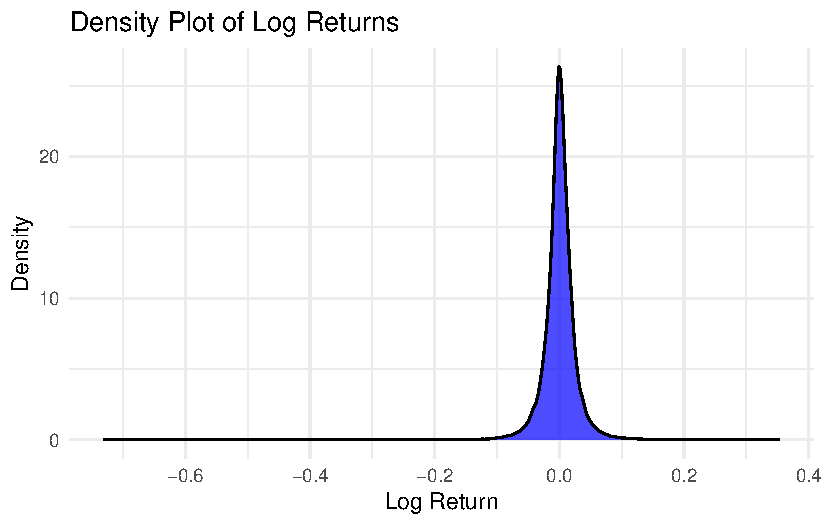
\includegraphics{Lab4_files/figure-pdf/problem 2-1.pdf}

\begin{Shaded}
\begin{Highlighting}[]
  \FunctionTok{ggplot}\NormalTok{(stocks\_ratio, }\FunctionTok{aes}\NormalTok{(}\AttributeTok{x =}\NormalTok{ log\_return)) }\SpecialCharTok{+}
  \FunctionTok{geom\_histogram}\NormalTok{(}\AttributeTok{bins =} \DecValTok{50}\NormalTok{, }\AttributeTok{fill =} \StringTok{"blue"}\NormalTok{, }\AttributeTok{alpha =} \FloatTok{0.7}\NormalTok{) }\SpecialCharTok{+}
  \FunctionTok{labs}\NormalTok{(}\AttributeTok{title =} \StringTok{"Histogram of Log Returns"}\NormalTok{, }\AttributeTok{x =} \StringTok{"Log Return"}\NormalTok{, }\AttributeTok{y =} \StringTok{"Frequency"}\NormalTok{) }\SpecialCharTok{+}
  \FunctionTok{theme\_minimal}\NormalTok{()}
\end{Highlighting}
\end{Shaded}

\begin{verbatim}
Warning: Removed 14 rows containing non-finite outside the scale range
(`stat_bin()`).
\end{verbatim}

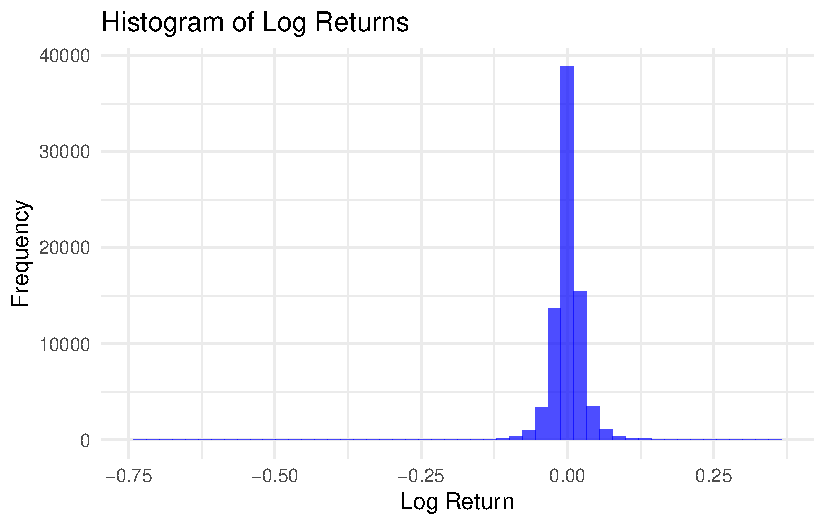
\includegraphics{Lab4_files/figure-pdf/problem 2-2.pdf}

\begin{Shaded}
\begin{Highlighting}[]
  \FunctionTok{ggplot}\NormalTok{(stocks\_ratio, }\FunctionTok{aes}\NormalTok{(}\AttributeTok{sample =}\NormalTok{ log\_return)) }\SpecialCharTok{+}
  \FunctionTok{geom\_qq}\NormalTok{() }\SpecialCharTok{+}
  \FunctionTok{geom\_qq\_line}\NormalTok{(}\AttributeTok{color =} \StringTok{"red"}\NormalTok{) }\SpecialCharTok{+}
  \FunctionTok{labs}\NormalTok{(}\AttributeTok{title =} \StringTok{"QQ{-}Plot of Log Returns"}\NormalTok{, }\AttributeTok{x =} \StringTok{"Theoretical Quantiles"}\NormalTok{, }\AttributeTok{y =} \StringTok{"Sample Quantiles"}\NormalTok{) }\SpecialCharTok{+}
  \FunctionTok{theme\_minimal}\NormalTok{()}
\end{Highlighting}
\end{Shaded}

\begin{verbatim}
Warning: Removed 14 rows containing non-finite outside the scale range
(`stat_qq()`).
\end{verbatim}

\begin{verbatim}
Warning: Removed 14 rows containing non-finite outside the scale range
(`stat_qq_line()`).
\end{verbatim}

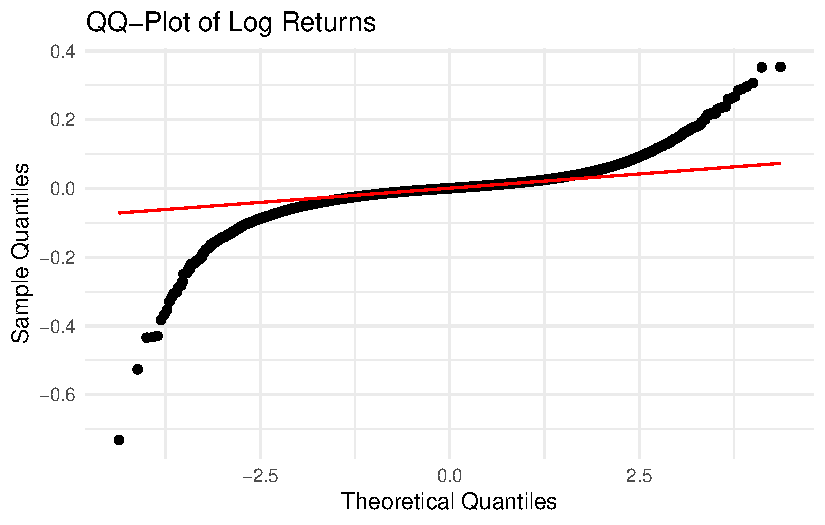
\includegraphics{Lab4_files/figure-pdf/problem 2-3.pdf}

\textbf{\emph{There appear to be some extreme outliers at the edges of
the QQ-plot, which are difficult to discern from the density plots. This
QQ-plot reminds me of data related to crashes and the timing of
accidents, but I don't believe this dataset is circular. Could these
patterns suggest some seasonality, such as volatility around quarterly
releases or extreme market shifts?}\\
\strut \\
\strut \\
Problem 3:} Volume measures how many shares were traded of a given stock
over a set time period, and high volume days often associate with
important events or market dynamics.

\begin{itemize}
\item
  Make a scatter plot of \texttt{volume} versus \texttt{log\_return},
  faceted by symbol to account for the fact that different stocks have
  different trading volumes. Do you see an association between volume
  and log\_return in these scatter plots?
\item
  Use the \texttt{cor} function to compute the pearson's correlation
  coefficient between \texttt{volume} and \texttt{log\_return} for each
  symbol. Why do you think the correlations are close to 0?
\end{itemize}

Hint: use it with summarize and don't forget that cor is a base R
function so you will either need to filter NA values for volume and
log\_return or appropriately choose the \texttt{use} flag in the
argument- see ?cor for more info.

\begin{itemize}
\item
  Next compute the correlation in the same manner but this time
  transform log\_return using the absolute value function. Recreate the
  faceted scatter-plots from the first part of the problem but with the
  absolute-value transformed log\_return. How have the correlations
  changed from the previous summary?

\begin{Shaded}
\begin{Highlighting}[]
\CommentTok{\#A}
\NormalTok{stocks\_ratio }\SpecialCharTok{|\textgreater{}}
  \FunctionTok{ggplot}\NormalTok{(}\FunctionTok{aes}\NormalTok{(}\AttributeTok{y =}\NormalTok{ volume, }\AttributeTok{x =}\NormalTok{ log\_return)) }\SpecialCharTok{+}
  \FunctionTok{geom\_point}\NormalTok{(}\AttributeTok{alpha =} \FloatTok{0.3}\NormalTok{) }\SpecialCharTok{+}
  \FunctionTok{facet\_wrap}\NormalTok{(}\SpecialCharTok{\textasciitilde{}}\NormalTok{ symbol, }\AttributeTok{scales =} \StringTok{"free\_y"}\NormalTok{, }\AttributeTok{ncol=}\DecValTok{3}\NormalTok{) }\SpecialCharTok{+}
  \FunctionTok{labs}\NormalTok{(}\AttributeTok{title =} \StringTok{"Scatter Volume vs. Log Return"}\NormalTok{,}
       \AttributeTok{y =} \StringTok{"Volume"}\NormalTok{,}
       \AttributeTok{x =} \StringTok{"Log Return"}\NormalTok{) }\SpecialCharTok{+}

  \FunctionTok{theme\_minimal}\NormalTok{()}
\end{Highlighting}
\end{Shaded}

\begin{verbatim}
Warning: Removed 14 rows containing missing values or values outside the scale range
(`geom_point()`).
\end{verbatim}

  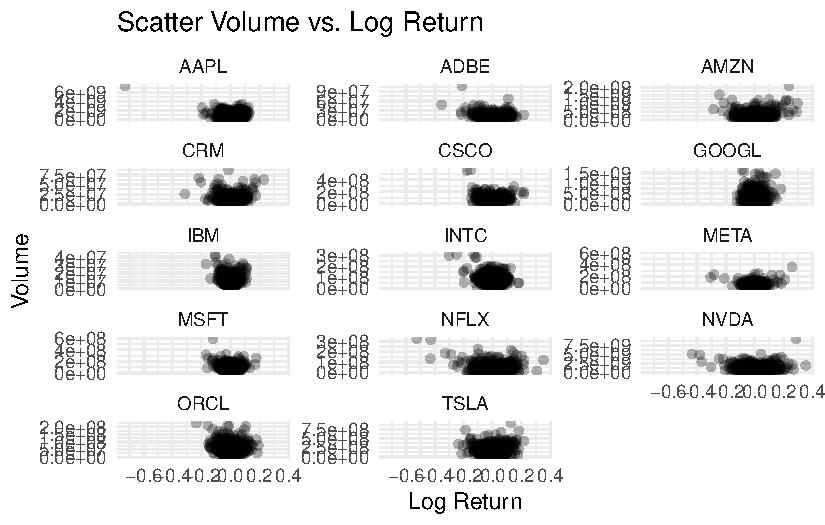
\includegraphics{Lab4_files/figure-pdf/problem3-1.pdf}

\begin{Shaded}
\begin{Highlighting}[]
\CommentTok{\#B}
\NormalTok{correlation\_results }\OtherTok{\textless{}{-}}\NormalTok{ stocks\_ratio }\SpecialCharTok{|\textgreater{}}
  \FunctionTok{group\_by}\NormalTok{(symbol) }\SpecialCharTok{|\textgreater{}}
  \FunctionTok{summarize}\NormalTok{(}
    \AttributeTok{correlation =} \FunctionTok{cor}\NormalTok{(volume, log\_return, }\AttributeTok{use =} \StringTok{"complete.obs"}\NormalTok{),}
    \AttributeTok{.groups =} \StringTok{\textquotesingle{}drop\textquotesingle{}}
\NormalTok{  )}

\FunctionTok{print}\NormalTok{(correlation\_results)}
\end{Highlighting}
\end{Shaded}

\begin{verbatim}
# A tibble: 14 x 2
   symbol correlation
   <chr>        <dbl>
 1 AAPL       -0.0780
 2 ADBE       -0.0801
 3 AMZN        0.0828
 4 CRM         0.0207
 5 CSCO       -0.0589
 6 GOOGL       0.0280
 7 IBM        -0.0703
 8 INTC       -0.0870
 9 META        0.0292
10 MSFT       -0.0579
11 NFLX       -0.0548
12 NVDA        0.0173
13 ORCL       -0.0428
14 TSLA        0.0619
\end{verbatim}

\begin{Shaded}
\begin{Highlighting}[]
\NormalTok{correlation\_abs\_results }\OtherTok{\textless{}{-}}\NormalTok{ stocks\_ratio }\SpecialCharTok{|\textgreater{}}
  \FunctionTok{group\_by}\NormalTok{(symbol) }\SpecialCharTok{|\textgreater{}}
  \FunctionTok{summarize}\NormalTok{(}
    \AttributeTok{correlation\_abs =} \FunctionTok{cor}\NormalTok{(volume, }\FunctionTok{abs}\NormalTok{(log\_return), }\AttributeTok{use =} \StringTok{"complete.obs"}\NormalTok{),}
    \AttributeTok{.groups =} \StringTok{\textquotesingle{}drop\textquotesingle{}}
\NormalTok{  )}
\FunctionTok{print}\NormalTok{(correlation\_abs\_results)}
\end{Highlighting}
\end{Shaded}

\begin{verbatim}
# A tibble: 14 x 2
   symbol correlation_abs
   <chr>            <dbl>
 1 AAPL             0.454
 2 ADBE             0.562
 3 AMZN             0.579
 4 CRM              0.547
 5 CSCO             0.540
 6 GOOGL            0.363
 7 IBM              0.596
 8 INTC             0.434
 9 META             0.549
10 MSFT             0.489
11 NFLX             0.519
12 NVDA             0.513
13 ORCL             0.520
14 TSLA             0.462
\end{verbatim}

\begin{Shaded}
\begin{Highlighting}[]
\CommentTok{\#C}
\NormalTok{stocks\_ratio }\SpecialCharTok{|\textgreater{}}
  \FunctionTok{ggplot}\NormalTok{(}\FunctionTok{aes}\NormalTok{(}\AttributeTok{y =}\NormalTok{ volume, }\AttributeTok{x =} \FunctionTok{abs}\NormalTok{(log\_return))) }\SpecialCharTok{+}
  \FunctionTok{geom\_point}\NormalTok{(}\AttributeTok{alpha =} \FloatTok{0.3}\NormalTok{) }\SpecialCharTok{+}
  \FunctionTok{facet\_wrap}\NormalTok{(}\SpecialCharTok{\textasciitilde{}}\NormalTok{ symbol, }\AttributeTok{scales =} \StringTok{"free\_y"}\NormalTok{, }\AttributeTok{ncol=}\DecValTok{3}\NormalTok{) }\SpecialCharTok{+}
  \FunctionTok{labs}\NormalTok{(}\AttributeTok{title =} \StringTok{"Scatter Volume vs. abslute Log Return"}\NormalTok{,}
       \AttributeTok{y =} \StringTok{"Volume"}\NormalTok{,}
       \AttributeTok{x =} \StringTok{"Log Return"}\NormalTok{) }\SpecialCharTok{+}

  \FunctionTok{theme\_minimal}\NormalTok{()}
\end{Highlighting}
\end{Shaded}

\begin{verbatim}
Warning: Removed 14 rows containing missing values or values outside the scale range
(`geom_point()`).
\end{verbatim}

  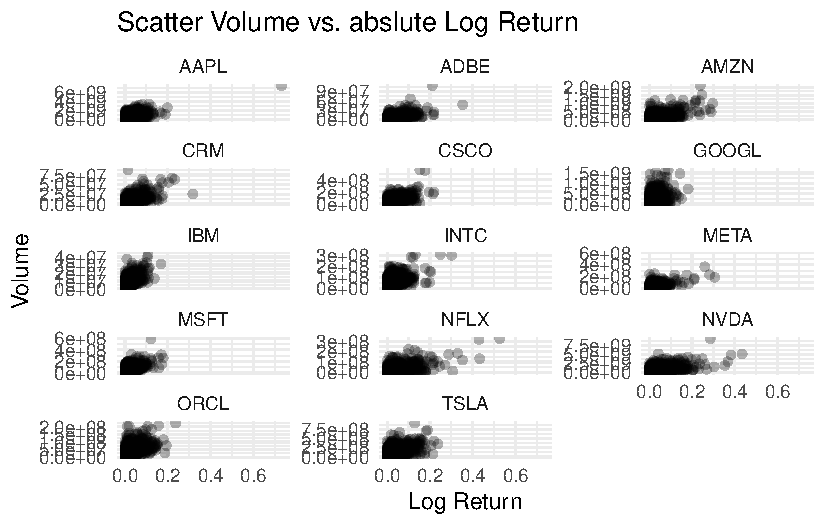
\includegraphics{Lab4_files/figure-pdf/problem3-2.pdf}

  \textbf{\emph{The absolute function on log returns removed the
  negative values, allowing us to focus on how volume correlated with
  changes in return. For instance, we can now see how much Apple traded
  whenever there was a 3\% change in return. This comparison effectively
  highlights the relationship between trading volume and price changes.
  The scatter plot for absolute log returns illustrates this well; I can
  almost visualize it as if I took the original scatter facet plot and
  folded it vertically along the 0.0 line of the log return variable.}}
\end{itemize}

\textbf{Problem 4:} For this problem we will implement a more
complicated mathematical transformation of data by calculating a measure
of liquidity for each stock.

Liquidity is defined loosely as the ability for a given asset to be
bought or sold without a large impact on price. Liquid assets can be
bought and sold quickly and easily, whereas illiquid assets have large
increases or decreases in their price when someone tries to buy or sell
them in large quantities. Liquidity is considered an important property
of a well functioning financial market, and declines in liquidity have
been blamed for worsening or triggering stock market crashes.

Many methods have been invented to measure liquidity, but for this
problem we will focus on a method called ``Kyle's \(\lambda\)''. Kyle's
\(\lambda\) estimates liquidity by using a linear regression between the
absolute value daily return of a stock and the logarithm of the dollar
volume of that stock. The time periods used to estimate this regression
can vary, but here we will use daily returns and a one month time period
(defined as 20 trading days). You will learn a lot about linear models
in DATA 606 and other classes, but to be complete, \(\lambda\) is a
coefficient in the following linear model: \[
|R_t-1| = c + \lambda \log((\mathrm{Volume})_t (\mathrm{close})_t) + \epsilon_t
\] where the coefficients \(c\) and \(\lambda\) will be calculated to
minimize the error \(\epsilon_t\) over the past 20 trading days.

\(\lambda\) stands for the amount that the stock price will move in
units of basis points for a given \(\log\) dollar volume of trade. A
small \(\lambda\) indicates high liquidity, and a high \(\lambda\)
indicates low liquidity.

\(\lambda\) can be be calculated using rolling averages on the time
series data with the \texttt{TTR} package, specifically the function
\texttt{runMean} which when used within a \texttt{dplyr} pipeline will
calculate the mean over the past \(n\) data points. For example, the
command:

\begin{Shaded}
\begin{Highlighting}[]
\FunctionTok{library}\NormalTok{(TTR)}
\NormalTok{stocks\_ratio }\SpecialCharTok{|\textgreater{}} \FunctionTok{group\_by}\NormalTok{(symbol) }\SpecialCharTok{|\textgreater{}}  \FunctionTok{mutate}\NormalTok{(}\AttributeTok{log\_return\_20d =} \FunctionTok{runMean}\NormalTok{(log\_return,}\AttributeTok{n=}\DecValTok{20}\NormalTok{))}
\end{Highlighting}
\end{Shaded}

adds a new variable which is equal to the mean of the log\_return over
the past 20 days. The mathematical formula for \(\lambda\) is: \[
\lambda = \frac{\mathrm{mean}(R_a\log( p_c V ))
- \mathrm{mean}\left(R_a\right) \mathrm{mean}\left(\log\left(p_c V\right) \right) }
{\mathrm{mean}\left(\log\left( p_c V \right)^2\right)
-\mathrm{mean}\left(\log(p_c V)\right)^2 }
\] where to make the formula easier to read we have defined
\(R_a = |\mathrm{return} -1|\), \(p_c = \mathrm{close}\) and
\(V = \mathrm{volume}\), and the averages have been taken over the past
20 days of data.

\begin{Shaded}
\begin{Highlighting}[]
\NormalTok{stocks\_ratio }\OtherTok{\textless{}{-}}\NormalTok{ stocks\_ratio }\SpecialCharTok{|\textgreater{}}
  \FunctionTok{group\_by}\NormalTok{(symbol) }\SpecialCharTok{|\textgreater{}}
  \FunctionTok{mutate}\NormalTok{(}
    
    \AttributeTok{R\_a =} \FunctionTok{abs}\NormalTok{(daily\_return }\SpecialCharTok{{-}} \DecValTok{1}\NormalTok{),  }
    \AttributeTok{p\_c\_V =}\NormalTok{ (volume }\SpecialCharTok{*}\NormalTok{ close),  }
    \AttributeTok{kyle =}\NormalTok{ (}\FunctionTok{runMean}\NormalTok{(R\_a }\SpecialCharTok{*}\FunctionTok{log}\NormalTok{(p\_c\_V),}\AttributeTok{n=}\DecValTok{20}\NormalTok{ ) }\SpecialCharTok{{-}}
                \FunctionTok{runMean}\NormalTok{(R\_a,}\AttributeTok{n=}\DecValTok{20}\NormalTok{ ) }\SpecialCharTok{*} \FunctionTok{runMean}\NormalTok{(}\FunctionTok{log}\NormalTok{(p\_c\_V),}\AttributeTok{n=}\DecValTok{20}\NormalTok{)) }
              \SpecialCharTok{/} 
\NormalTok{             (}
               \FunctionTok{runMean}\NormalTok{(}
\NormalTok{                 (}\FunctionTok{log}\NormalTok{(p\_c\_V)}\SpecialCharTok{\^{}}\DecValTok{2}\NormalTok{),}\AttributeTok{n=}\DecValTok{20}\NormalTok{) }\SpecialCharTok{{-}}
\NormalTok{                 (}
                   \FunctionTok{runMean}\NormalTok{(}
                     \FunctionTok{log}\NormalTok{(p\_c\_V ),}\AttributeTok{n=}\DecValTok{20}\NormalTok{)}\SpecialCharTok{\^{}}\DecValTok{2}\NormalTok{)  }
\NormalTok{  )}
\NormalTok{  )}\SpecialCharTok{|\textgreater{}}
  \FunctionTok{ungroup}\NormalTok{()}
\end{Highlighting}
\end{Shaded}

\begin{itemize}
\item
  Add a new variable called \texttt{kyle} to the data frame by
  implementing the above formula for \(\lambda\). Make sure to read and
  implement the formula very carefully, and to use the \texttt{runMean}
  function to calculate the rolling average correctly.
\item
  Plot Kyle's lambda for each stock over time (I would use a faceted
  scatterplot). What do you notice about how this measure of liquidity
  behaves (remember liquidity is high when \(\lambda\) is small)?\\
  \strut \\
  \textbf{\emph{Should i have negative values for kyle?\\
  I think this wrong but i dont see my error at this point,}}

\begin{Shaded}
\begin{Highlighting}[]
\NormalTok{stocks\_ratio }\SpecialCharTok{|\textgreater{}} 
  \FunctionTok{ggplot}\NormalTok{(}\FunctionTok{aes}\NormalTok{(}\AttributeTok{x =}\NormalTok{ date, }\AttributeTok{y =}\NormalTok{ kyle)) }\SpecialCharTok{+}
  \FunctionTok{geom\_point}\NormalTok{(}\AttributeTok{alpha =} \FloatTok{0.3}\NormalTok{) }\SpecialCharTok{+}
  \FunctionTok{facet\_wrap}\NormalTok{(}\SpecialCharTok{\textasciitilde{}}\NormalTok{ symbol, }\AttributeTok{scales =} \StringTok{"free\_y"}\NormalTok{, }\AttributeTok{ncol=}\DecValTok{3}\NormalTok{) }\SpecialCharTok{+}
  \FunctionTok{labs}\NormalTok{(}\AttributeTok{title =} \StringTok{"Kyle\textquotesingle{}s Lambda Over Time for Each Stock"}\NormalTok{,}
       \AttributeTok{x =} \StringTok{"Date"}\NormalTok{, }
       \AttributeTok{y =} \StringTok{"Kyle\textquotesingle{}s Lambda"}\NormalTok{) }\SpecialCharTok{+}
  \FunctionTok{theme\_minimal}\NormalTok{()}
\end{Highlighting}
\end{Shaded}

\begin{verbatim}
Warning: Removed 280 rows containing missing values or values outside the scale range
(`geom_point()`).
\end{verbatim}

  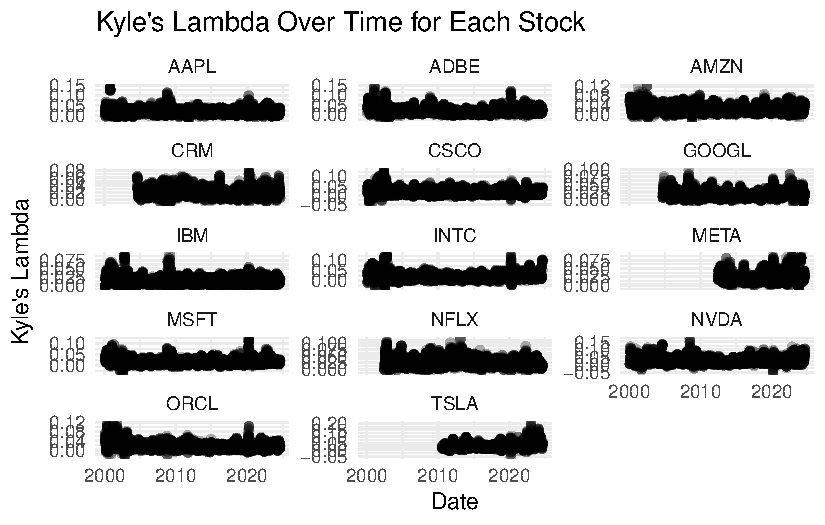
\includegraphics{Lab4_files/figure-pdf/unnamed-chunk-4-1.pdf}

  \textbf{\emph{Again, i am not sure about the -kyle values but as far
  as i can see the higher the kyle the less amount of trading at that
  time.}}
\item
  Next add a new variable to the dataframe called \texttt{extreme} which
  is true when the log\_return for a given stock is \emph{either}
  greater than 95\% of other values of the log\_return \emph{or} less
  than 95\% of all values of log\_return. Use the \texttt{percent\_rank}
  \texttt{dplyr} window function along with logical operators to create
  this variable. Then for each stock calculate the mean value of Kyle's
  lambda for the days when the log\_return had extreme values and for
  when it didn't (as identified by the \texttt{extreme} variable). What
  do your calculations and figures indicate about liquidity during
  extreme events?
\end{itemize}

\begin{Shaded}
\begin{Highlighting}[]
\NormalTok{stocks\_ratio }\OtherTok{\textless{}{-}}\NormalTok{ stocks\_ratio }\SpecialCharTok{|\textgreater{}} 
  \FunctionTok{group\_by}\NormalTok{(symbol) }\SpecialCharTok{|\textgreater{}} 
  \FunctionTok{mutate}\NormalTok{(}
    
    \AttributeTok{extreme =} \FunctionTok{percent\_rank}\NormalTok{(log\_return) }\SpecialCharTok{\textgreater{}} \FloatTok{0.95} \SpecialCharTok{|} \FunctionTok{percent\_rank}\NormalTok{(log\_return) }\SpecialCharTok{\textless{}} \FloatTok{0.05}
\NormalTok{  ) }\SpecialCharTok{|\textgreater{}}
  \FunctionTok{ungroup}\NormalTok{()}

\NormalTok{kyles\_mean }\OtherTok{\textless{}{-}}\NormalTok{ stocks\_ratio }\SpecialCharTok{|\textgreater{}} 
  \FunctionTok{group\_by}\NormalTok{(symbol, extreme) }\SpecialCharTok{|\textgreater{}} 
  \FunctionTok{summarize}\NormalTok{(}\AttributeTok{mean\_kyle =} \FunctionTok{mean}\NormalTok{(kyle, }\AttributeTok{na.rm =} \ConstantTok{TRUE}\NormalTok{)) }\SpecialCharTok{|\textgreater{}}
  \FunctionTok{ungroup}\NormalTok{()}
\end{Highlighting}
\end{Shaded}

\begin{verbatim}
`summarise()` has grouped output by 'symbol'. You can override using the
`.groups` argument.
\end{verbatim}

\begin{Shaded}
\begin{Highlighting}[]
\NormalTok{kyles\_mean}
\end{Highlighting}
\end{Shaded}

\begin{verbatim}
# A tibble: 42 x 3
   symbol extreme mean_kyle
   <chr>  <lgl>       <dbl>
 1 AAPL   FALSE      0.0203
 2 AAPL   TRUE       0.0308
 3 AAPL   NA       NaN     
 4 ADBE   FALSE      0.0194
 5 ADBE   TRUE       0.0366
 6 ADBE   NA       NaN     
 7 AMZN   FALSE      0.0240
 8 AMZN   TRUE       0.0356
 9 AMZN   NA       NaN     
10 CRM    FALSE      0.0204
# i 32 more rows
\end{verbatim}

\textbf{\emph{The figures suggest that liquidity decreases during
extreme events, meaning that it becomes more difficult to buy or sell
assets without significantly impacting their price.\\
\strut \\
}}



\end{document}
